%%This is a very basic article template.
%%There is just one section and two subsections.
\documentclass[english,a4paper]{scrartcl}

\usepackage{graphicx}
\usepackage{listings}
\usepackage{color}
\usepackage{makeidx}
\usepackage{hyperref}
\usepackage{parskip}
\usepackage{multirow}
\usepackage{tocloft}
\renewcommand{\cftsecaftersnumb}{\hspace{6em}}
\renewcommand{\cftsubsecaftersnumb}{\hspace{6em}}
\renewcommand{\cftsubsubsecaftersnumb}{\hspace{6em}}

\makeindex

\hypersetup{
    %bookmarks=true,         % show bookmarks bar?
    unicode=false,          % non-Latin characters in Acrobat’s bookmarks
    pdftoolbar=true,        % show Acrobat’s toolbar?
    pdfmenubar=true,        % show Acrobat’s menu?
    pdffitwindow=false,     % window fit to page when opened
    pdfstartview={FitH},    % fits the width of the page to the window
    pdftitle={TDT4205 Compilers - Exercise 4 - hvatum},    % title
    pdfauthor={Stian Hvatum},     % author
    pdfsubject={TDT4205 Compilers},   % subject of the document
    pdfcreator={Stian Hvatum},   % creator of the document
    pdfproducer={Stian Hvatum}, % producer of the document
    pdfnewwindow=true,      % links in new window
    colorlinks,       % false: boxed links; true: colored links
    linkcolor=black,          % color of internal links
    citecolor=green,        % color of links to bibliography
    filecolor=magenta,      % color of file links
    urlcolor=cyan           % color of external links
}

\definecolor{listinggray}{gray}{0.9}
\definecolor{lbcolor}{rgb}{0.9,0.9,0.9}
\lstset{
    keywordstyle=\bfseries\ttfamily\color[rgb]{0,0,1},
    identifierstyle=\ttfamily,
    commentstyle=\color[rgb]{0.133,0.545,0.133},
    stringstyle=\ttfamily\color[rgb]{0.627,0.126,0.941},
    showstringspaces=false,
    basicstyle=\tiny,
    numberstyle=\tiny,
    framexleftmargin=3pt,
    numbers=left,
    stepnumber=1,
    numbersep=15pt,
    tabsize=2,
    breaklines=true,
    prebreak = \raisebox{0ex}[0ex][0ex]{\ensuremath{\hookleftarrow}},
    breakatwhitespace=false,
    aboveskip={1.5\baselineskip},
    columns=fixed,
    upquote=true,
    extendedchars=true,
  	frame=l,
    sensitive=true,
}
\lstdefinelanguage{vsl}
  {morekeywords={FUNC,VAR,PRINT},
  sensitive=false,
  morecomment=[l]{//},
  morecomment=[s]{/*}{*/},
  morestring=[b]",
}


\renewcommand{\thesection}{PART \arabic{section}}
\renewcommand{\thesubsection}{Task \arabic{section}.\arabic{subsection}}
\renewcommand{\thesubsubsection}{\arabic{subsubsection}.}

\title{TDT4205 Compilers\\
\Huge Exercise 4}
\author{Stian Hvatum (hvatum)\\MTDT}

\begin{document}
\maketitle
\tableofcontents
\section{Theory and Assembly Programming}
\subsection{Stack Frames}
\subsubsection{What is a stack frame}
A \emph{stack frame} is a location in a programs logical memory, or more
precicely, a location on the \emph{stack}, where a function keeps its current
local variables. The stack frame grows as local variables are added, and shrinks
as they are poped of, eg. if they are not going to be used any more.

\subsubsection{Stack frame illustration}
\centerline{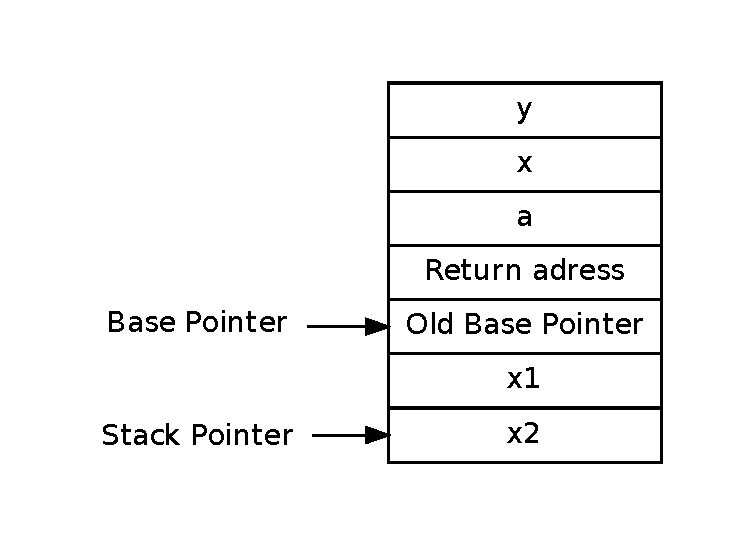
\includegraphics[width=300px]{stackframe.pdf}}
Here we see a model of a stack frame at the top of the program stack. The stack
grows downwards, so a new variable will be placed below x2. In that case, the
stack pointer would be decreased accordingly. Each block will have a size
of 4 bytes, given a 32-bit system.

\subsubsection{Setting up and tearing down stack frames}
To call a function, the caller will put the functions arguments on the top of
its stack, and then call the function. This way, a function will always find its
arguments right above its stack frame. After the function call, we need to
increment the stack pointer to ``clean'' the stack of the call arguments. The
top of the stack is pointed to by the \$esp-register, and the stack base is
pointed to by the \$ebp-register.
\begin{lstlisting}[language={[x86masm]Assembler}]
	/* Call printf(string, l_var_1) */
	pushl   -4(%ebp)
	pushl   $.STRING0
	call    printf

	/* Clean up on stack */
	addl    $8, %esp
\end{lstlisting}

When a function is called it is itself responsible for setting up and tearing
down its own stack frame.  The function will do the following statements to set up the
stack frame:
\begin{lstlisting}[language={[x86masm]Assembler}]
func:
    /* Store old base pointer on top of stack */
    pushl   %ebp

    /* Set new stack base (ebp) to old top-of-stack (esp) */
    movl    %esp, %ebp
\end{lstlisting}
Here we see that the function pushes the old base to the top of the stack, so
that it know how to restore the previous stack frame on return. It also creates
its own base by setting the stack base to point at the old
top of stack. Now, base and top is at the same location, and we basically have
our new stack frame, with base, stack pointer and function arguments. New local
variables will be placed at the position below the stack pointer, and then the
stack pointer is decremented with the size of the variable. Typically 4 bytes.

To  return to the caller, the function will have to tear down its own stack. We
state {\ttfamily leave} to tear down our own stack frame, and {\ttfamily ret} to
return to the point where the current function was called. We see that in
x86-assembly, the stack operations are supported by 

\begin{lstlisting}[language={[x86masm]Assembler}]
	/* Clean up stack frame */
	leave

	/* Return home */
	ret
\end{lstlisting}
Now, we are back at the caller, who must remember to clean the stack of the
arguments, as stated above. We must also notice that a function may alter the
registers to its need, so before calling a function, we must store the
registers that keeps usefull values, else the values may be lost.

Notes:
{\ttfamily leave} is equivalent
to\footnote{\url{http://en.wikipedia.org/wiki/X86_instruction_listings}}
\begin{lstlisting}[language={[x86masm]Assembler}]
	mov %esp, %ebp
	pop %ebp
\end{lstlisting}
and the stack-setup could also be done utilitizing the {\ttfamily
enter}-command.

\newpage
\subsection{x86 Assembly Programming}
The complete file \emph{foo.s} is attached with the delivery of this file. This
is the function I have implemented:
\begin{lstlisting}[language={[x86masm]Assembler}]
foo:
    /* Store old base pointer on top of stack */
    pushl   %ebp

    /* Set new stack base (ebp) to old top-of-stack (esp) */
    movl    %esp, %ebp

    /* Store 0 in ecx  (loop starts at 1, but is incremented in first test) */
    movl    $0,   %ecx

    /* Store 0 on the stack, our sum value */
    pushl   $0

    /* And start loop-test */
    jmp tst_lp

lbody:
    /* Loop body */
    /* Modulo = divide and check rest-register */


    /* Check for input divisible by 3 */
    movl    %ecx, %eax
    movl    $3,   %ebx
    cdq
    idiv    %ebx
    /* edx now contains ecx mod 3 */
    cmp     $0,   %edx
    jz tst_ok /* Test true */

     /* Check for input divisible by 5 */
    movl    %ecx, %eax
    movl    $5,   %ebx
    cdq
    idiv    %ebx
    /* edx now contains ebx mod 5 */
    cmp     $0,   %edx
    jnz tst_lp /* Test false */
tst_ok:
    addl    %ecx, -4(%ebp)
    
tst_lp:
    /* Get the function argument and store in ebx */
    movl    8(%ebp), %ebx

    /* Increment and test */ 
    inc %ecx
    /* if ebx < ecx => jump to start of loop */
    cmp %ebx, %ecx
    jl lbody

    pushl -4(%ebp)
    /* Print results */
    /* sum is on top of stack */
    pushl   $.STRING0
    call    printf

    /* Clean up on stack */
    addl    $8, %esp
    /* Clean up stack frame */
    leave

    /* Return home */
    ret
\end{lstlisting}
\newpage
\subsection{Symbol Tables}
\subsubsection{Stack offset}
\begin{description}
\item[a] -4
\item[b] -8
\item[c] -28\\since previous started at -8 and offset is 5 times the size of 4
bytes.\\Mathematically: $-8 - (4 \cdot 5) = -8 - 20 = -28$
\end{description}

\subsubsection{Lexical depth}
We need to know the lexical depth of a symbol in order to get to the right
symbol in the current scope. I give you an example:
\begin{lstlisting}[language=vsl]
FUNC depth_printer() {
	VAR a;
	a = 1;
	{
		PRINT a;
		VAR a;
		a = 2;
		PRINT a;
	}
	PRINT a;
}
\end{lstlisting}
If we are to know inside the scope at line 4-9 which variable to print at first
and last {\ttfamily PRINT}, we need to know what lexical depth we are in, and
what variables are available to us. It may be more important at the last print
(on line 10), since the inner variable {\ttfamily a = 2} is more recent than
{\ttfamily a = 1}, and thus we would print 2 if we were not aware of lexical
depth. If we just knew the offset on the stack frame, we would not know what
variable to use in each print, as we would not be aware of scope, and would
possibly print the wrong variable.
\printindex
\end{document}
